\section{The Qubit}

As we have already described in a previous section, qubits are the fundamental units of measuring
the information contents of a quantum system. In classical terms, computers use two voltage levels
to represent the two states of a bit: choosing arbitrarily, +0V for the zero state and +5V for the
one state. Quantum systems map those logical states of qubits to some physical property of the quantum
system, which can be its spin, for electrons, or its polarity, for photons. Mathematically we represent
those states (0 and 1) with the \textit{unit vectors} $\ket{0}$ and $\ket{1}$ which constitute the
computational basis.

These basis are complex vectors $\ket{0},\ket{1}\in\mathbb{H}^2$ and are written as:

\begin{align}
    \ket{0}=\begin{bmatrix}
        1\\
        0
    \end{bmatrix}
    \text{ and }
    &
    \ket{1}=\begin{bmatrix}
        0\\
        1
    \end{bmatrix}
\end{align}

The big difference from the classical bit is that qubits are a superposition of some two basis states.
Although this is a very interesting phenomenon, computation constitutes that at some point we would need
to output/read the result. We have to remind at this point that this would constitute a measurement and
the qubit would have to \say{collapse} to one of the two basis states with a probability equal to
the square of the probability amplitude of that basis state.

\subsection{The Bloch Sphere}

The Bloch sphere is an attempt to depict the state of qubit as a vector that originates from the center
of a sphere with a radius $r=1$.

Let $\ket{q}=q_0\ket{0}+q_1\ket{1}\in\mathbb{H}^2$ be a qubit with $q_0,q_1\in\mathbb{C}$ be
its probability amplitudes. We can parameterize those coefficients as:

\begin{align}
    q_0 = e^{i\gamma}\cos\frac{\theta}{2} &\hspace{2cm}
    q_1 = e^{i\delta}\sin\frac{\theta}{2}
\end{align}

We can now re-write the qubit $\ket{q}$ as:

\begin{equation}
    \ket{q}=e^{i\gamma}(\cos\frac{\theta}{2}\ket{0}+e^{i\phi}\sin\frac{\theta}{2}\ket{1})
\end{equation}

where $\phi=\gamma-\delta$. The \textit{global phase} $e^{i\gamma}$ is neglected most of the time
thus qubit $\ket{q}$ can be written as a matrix:

\begin{equation}
    \ket{q}=\begin{bmatrix}
        \cos\frac{\theta}{2}\\
        e^{i\phi}\sin\frac{\theta}{2}
    \end{bmatrix}
\end{equation}

To map the \emph{spherical coordinates} $(r,\phi,\theta)$ to cartesian coordinates we use the equalities:

\begin{gather}
    q_x=r\sin\theta\cos\phi\\
    q_y=r\sin\theta\sin\phi\\
    q_z=r\cos\theta
\end{gather}

So the qubit $\ket{q}$ can be plotted with coordinates $(q_x,q_y,q_z)$.

\begin{figure}[ht]
    \centering
    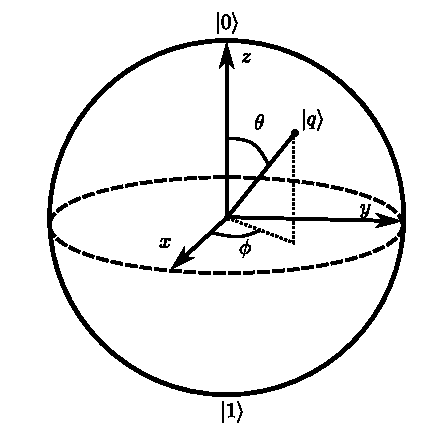
\includegraphics{images/3_Quantum_Computing/bloch_sphere.pdf}
    \caption{The Bloch sphere}
    \label{fig:bloch_sphere}
\end{figure}

We can note also the rest of the basis state that a qubit can have:

\begin{enumerate}
    \item along the $z$-axis we can distinguish the computational basis (see \ref{fig:bloch_sphere}): \begin{enumerate}
        \item $\ket{0}$ where the $+z$-axis crosses Bloch sphere's upper boundary
        \item $\ket{1}$ where the $-z$-axis crosses Bloch shpere's lower boundary
    \end{enumerate}
    \item along the $x$-axis: \begin{enumerate}
        \item at the cross section $+x$-axis where angles $\theta=\pi/2$ and $\phi=0$ we have the basis state $\ket{+}=\frac{\ket{0}+\ket{1}}{\sqrt{2}}$
        \item at the cross section $-x$-axis where angles $\theta=\pi/2$ and $\phi=\pi$ we have the basis state $\ket{-}=\frac{\ket{0}-\ket{1}}{\sqrt{2}}$
    \end{enumerate}
    \item along the $y$-axis: \begin{enumerate}
        \item at the cross section $+y$-axis where angles $\theta=\pi/2$ and $\phi=\pi/2$ we have the basis state $\ket{i+}$
        \item at the cross section $-y$-axis where angles $\theta=\pi/2$ and $\phi=3\pi/2$ we have the basis state $\ket{i-}$
    \end{enumerate}
\end{enumerate}

In this work we are going to be consered mostly with the computational basis states.